\documentclass{tufte-handout}

\usepackage{librecaslon}
\usepackage{fancyhdr}
\usepackage{hyperref}
\usepackage{tcolorbox} % needed for the text boxes
\usepackage{xcolor}
\usepackage{setspace}
\usepackage{graphics}
\usepackage{./tuftefoot}

% Set header and footer
\pagestyle{fancy}
\fancyhf{}
\lfoot{\includegraphics[height=1cm,keepaspectratio]{../img/i2i}}
\cfoot{\includegraphics[height=1cm,keepaspectratio]{../img/wb}}
\rfoot{\includegraphics[height=1cm,keepaspectratio]{../img/analytics}}

% Put checkbox to the left of the text
\def\LayoutCheckField#1#2{% label, field
	#2 #1%
}

% Line spacing
\onehalfspacing

% Define DIME Analytics visual identity colors
\definecolor{fontcolor}{HTML}{7A0569}

\titleformat{\section}%
{\Large\rmfamily\bf\color{fontcolor}}% format applied to label+text
{\llap{\colorbox{fontcolor}{\parbox{1.5cm}{\hfill\huge\color{fontcolor}\thesection}}}}% label
{2pt}% horizontal separation between label and title body
{}% before the title body
[]% after the title body

\titleformat{\subsection}%
{\large\rmfamily\color{fontcolor}}% format applied to label+text
{}% label
{1.5pt}% horizontal separation between label and title body
{}% before the title body
[]% after the title body

\newcommand{\dimeCheckBox}[1]{\CheckBox[height=0.01cm, width=0.4cm, bordercolor=gray]{#1}}
\newcommand{\dimeTextField}[3]{\TextField[name=#1, height=0.3cm, width=#2, bordercolor=gray]{#3}}


\newcommand{\titleBox}[1]{
	\begin{tcolorbox}
		[colframe = fontcolor,
		colback = fontcolor,
		sharp corners,
		halign = flush center,
		valign = center,
		height = 0.3\textwidth,
		after skip = 1cm]
		#1
	\end{tcolorbox}
}


% ------------------------------ End of preamble ---------------------------------------------
\begin{document}
	\begin{fullwidth}

\titleBox{
	\textcolor{white}{\LARGE{\textbf{DIME Analytics \\ Reproducibility Check Guidance Note}} \\
	\Large\textbf{{v2.0 - Last updated November 16, 2022}}}
}

	\section*{Reproducibility Check Guidance Note}

The reproducibility check verifies that the code package as submitted:

	\begin{enumerate}
		\setlength\itemsep{-0.1em}
		\item Is stable. It produces identical outputs each time it is run
		\item Produces outputs that exactly match the analytical outputs (tables and data visualizations) in the final manuscript, without manual adjustments
		\item Creates all the analytical outputs included in the final manuscript
	\end{enumerate}

	Computational reproducibility is mandatory for all working papers produced by DIME, and encouraged for other research outputs, such as briefs and reports. 

	Reproducibility checks are performed by DIME Analytics. Checks are typically completed within two weeks of submission of a functioning reproducibility package. DIME Analytics prepares a reproducibility review document which highlights any non-reproducible results, problematic practices, and stylistic improvements that would make the code easier to read. The check process is as follows.

	\subsection{1. \, Receving the reproducibility package}

	The research team requests a reproducibility check by emailing dimeanalytics@worldbank.org. The email must include the reproducibility package in a shared OneDrive or Dropbox folder, a GitHub repository, or a compressed folder sent by email if the files size allows. If using a World Bank GitHub repository, please share only the code files through GitHub and send the input data files using another channel. 
	
	The reproducibility package must contain the following:

	\bigskip

	\begin{itemize}
		\setlength\itemsep{-0.1em}
		\item \textbf{Code:} All scripts necessary to reproduce the analytical outputs of the paper, including a well-commented Master Script that allows to perform a one-button run of the code. If the reproducibility package runs in Stata and uses external commands, ado files must be included and the Master script should change the ado folder path accordingly.
		\item \textbf{Data:} All datasets necessary to run the master script. Data should be de-identified and public access; exceptions to this are handled with additional measures (see section \nameref{restricted-data} for details). The reproducibility package can include constructed datasets only, though conducting a review from earlier data preparation stages will facilitate data submission to journals\TFfootnotefw{AEA journals, for example, require reproducibility checks to begin with raw data.}.
		\item \textbf{Outputs\TFfootnotefw{The code, data and outputs should be stored in different subfolders.}:} All raw outputs used for the paper (tables and figures), as created by the master script.
		\item \textbf{Working Paper:} Final version of the paper; we will use this to compare the output generated by the code with the exhibits presented in the paper.
		\item \textbf{README.txt:} Text file delineating the requirements of the code and datasets included in the package, instructions about the directory structure DIME Analytics should follow, and any ad-hoc instructions to run the master script. See section \nameref{additional-resources} for a complete README template reference.
		\item \textbf{Completed Computational Reproducibility Checklist:} DIME Analytics ask submitting teams to provide \href{https://raw.githubusercontent.com/worldbank/dime-standards/master/dime-research-standards/pillar-3-research-reproducibility/checklists/Reproducibility%20package%20submission%20checklist.pdf}{this checklist} to verify all necessary components are included in the reproducibility package.
	\end{itemize}

	\subsection{2. \, Attempting a one-button run of the reproducibility package}

	\bigskip

	\begin{center}
		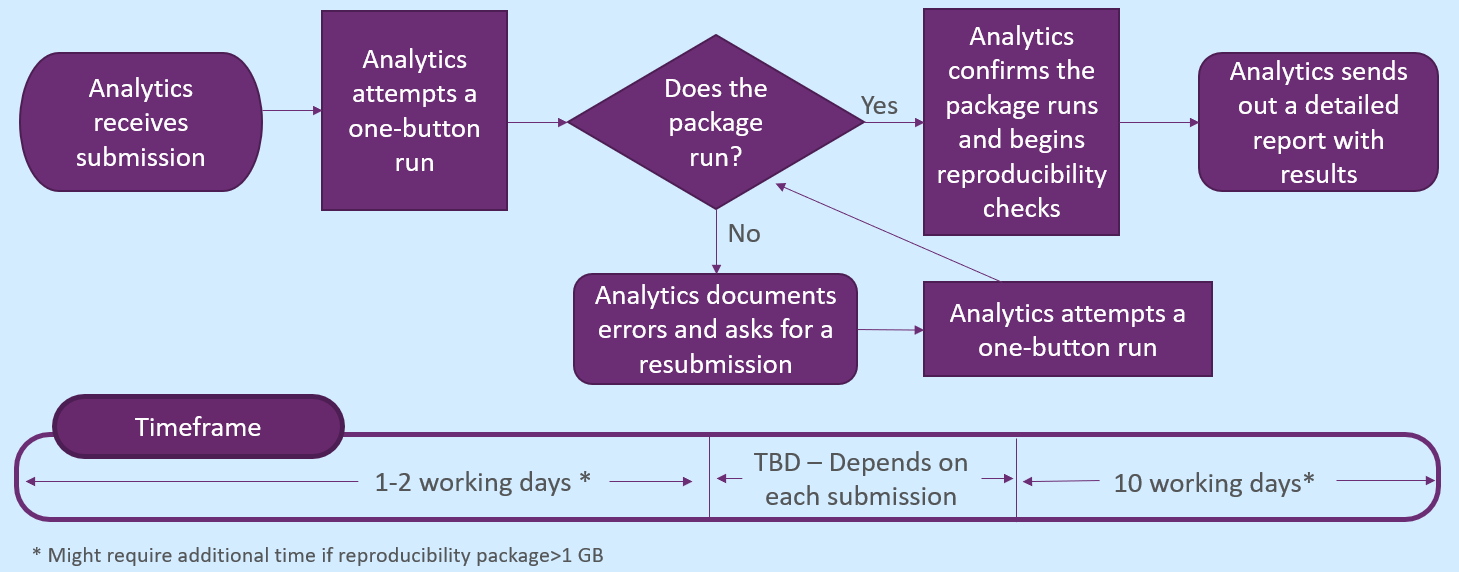
\includegraphics[width=0.9\linewidth]{../img/rep-checks-timeline.png}
	\end{center}

	\bigskip

	DIME Analytics changes the topmost global directory specified in the master script and attempts to run it – this is what is called a one-button run. The master script code should run without errors after adding the correct folder path of the computer where it will be running. For the paper to be considered fully reproducible, DIME Analytics should reproduce every exhibit in the paper showing analysis results through this push-button exercise. If the master script breaks, DIME Analytics will identify the point where it is breaking, document it, and attempt to make changes to continue with the review. If the corrections cannot be identified after a 15-minute check, the project team will be notified that further edits are required to conduct the reproducibility check.

	If the code runs from beginning to end, DIME Analytics verifies that the code produces every paper exhibit that shows analysis results. If the code is complete, DIME Analytics sends an email confirmation and provides the timeline for delivering the results of the review. Reproducibility checks take ten working days (two weeks) in most cases, but can take longer for computationally intensive packages, packages with more than 1 GB of total file size, or when a large volume of submissions is received.

	\subsection{3. \, Reproducibility check}

	After the one-button run works, DIME Analytics runs the following checks. A package must pass all checks for the working paper to be considered computationally reproducible. 

	\bigskip

	\begin{itemize}
		\setlength\itemsep{-0.1em}
		\item \textbf{Code completeness:} Every paper exhibit containing analysis results should be produced programatically by the code. Manual entry of values used in a table or plot, or point-and-click-generated exhibits are not in compliance with the computational reproducibility standard.
		\item \textbf{Output stability:} DIME Analytics will run the code between three to five times. Every output should be  identical across each run.
		\item \textbf{Computational reproducibility of tables:} Every statistic of every table needs to be consistent between the outputs produced by the code and the exhibits of the paper. Stable differences of less than 0.001 in point estimates and standard errors might not break adherence with DIME Reproducibility Standards and will be evaluated in a case-by-case basis to determine if they can occur for rounding differences due to hardware or system specifications.
		\item \textbf{Computational reproducibility of figures:} Every plot needs to be consistent between the code outputs and the paper figures. Differences in graph titles, x and y-axis titles, x and y-ticks, legends, and other style elements might not break adherence to DIME Research Standards, but DIME Analytics will document them in the results report.
	\end{itemize}

	\bigskip
	
	The results of the reproducibility check will be registered in two outputs.

	\bigskip

	\begin{enumerate}
		\setlength\itemsep{-0.1em}
		\item A report detailing the reproducibility status of each paper exhibit along with suggestions to increase code legibility or efficiency. An example can be found \href{https://github.com/worldbank/dime-standards/blob/master/dime-research-standards/pillar-3-research-reproducibility/DIME%20Analytics%20Reproducibility%20Check%20Comments%20example.pdf}{here}.
		\item A checklist with a summary of the results (example \href{https://raw.githubusercontent.com/worldbank/dime-standards/master/dime-research-standards/pillar-3-research-reproducibility/checklists/Reproducibility%20check%20result%20template.pdf}{here}).
	\end{enumerate}

	\bigskip

	\section*{Public release}

	Many journals require data and code to be made publicly available. Once the reproducibility checks are complete and the code and paper meet DIME Reproducibility Standards, DIME Analytics can help to organize a public release of using a repository on the World Bank GitHub (see section \nameref{additional-resources} for an example), the World Bank Microdata Catalog, or the World Bank Development Data Hub.

	\section{Additional resources}
	\label{additional-resources}

	\begin{itemize}
		\item \href{https://github.com/worldbank/rio-safe-space}{Reproducibility package example in a GitHub repository}
		\item \href{https://social-science-data-editors.github.io/template_README/template-README.html}{Template README of the Social Science Data Editors}
		\item \href{https://osf.io/agkmc}{Frequent reproducibility mistakes in Stata and how to avoid them}
	\end{itemize}

	\section{Restricted data}
	\label{restricted-data}

	If a reproducibility package must contain restricted or personal data, there are two options to conduct the reproducibility checks.

	\begin{enumerate}
		\item DIME Analytics can assist in setting up a data license agreement that specifies that one person from our team will have access to the data for the reproducibility checks during a limited time. Whether that is feasible will depend on the restrictions in any existing data agreement.
		\item DIME Analytics will verify reproducibility virtually. This usually entails granting the research team access to a VDI and setting a virtual meeting in which we verify that they copy the reproducibility package and run the code to produce the outputs. DIME Analytics will observe that it is reproducible, and then the team will delete all the data from the VDI. 
	\end{enumerate}

	\noindent
	Exceptions where none of these options are possible will be handled in a case by case basis.

	\end{fullwidth}
\end{document}
